\documentclass[lettersize,journal]{IEEEtran}
\usepackage{amsmath,amsfonts}
\usepackage{array}
\usepackage[caption=false,font=normalsize,labelfont=sf,textfont=sf]{subfig}
\usepackage{textcomp}
\usepackage{stfloats}
\usepackage{url}
\usepackage{graphicx}
\usepackage{cite}
\usepackage{booktabs}
\usepackage{multirow}

\graphicspath{{figures/}}
\newcommand{\paperfigurewidth}{\columnwidth}
\hyphenation{op-tical net-works semi-conduc-tor IEEE-Xplore Wind-rise}

\begin{document}

\title{Evidence-Grounded LLM Strategy Chains for Localized Wind Turbine Fault Operations and Maintenance}

\author{Yehong Dong
        and Shuai Hao
\thanks{This work studies localized knowledge construction and retrieval-augmented reasoning for wind turbine operations and maintenance.}
\thanks{Yehong Dong is with the School of New Energy, North China Electric Power University. Shuai Hao is with the School of Automation Science and Electrical Engineering, Beihang University (email: yehong.dong@example.com; shuai.hao@example.com).}}

\markboth{IEEE Transactions on Sustainable Energy,~Vol.~XX, No.~X, January~2026}%
{Dong \MakeLowercase{\textit{et al.}}: Evidence-Grounded LLM Strategy Chains for Wind Turbine O\&M}

\maketitle

\begin{abstract}
Wind turbine operations and maintenance (O\&M) relies on fault-code tables, manuals, repair records, and case reports whose meanings depend on turbine model and field context. Plain retrieval and large-language-model (LLM) assistants miss these scope constraints and produce answers that are difficult to audit. This paper presents a localized evidence-grounded O\&M reasoning framework with three algorithmic components---scope-bound fault-code retrieval, mechanism-closure graph construction, and verification-state strategy control---together with a deterministic intent-routing layer that resolves farm, model, and turbine-number queries without generation and defers under-specified fault queries for clarification. The framework converts heterogeneous documents into structured fault entries, wiki pages, a domain knowledge graph, and a mechanism-enhanced reasoning graph, and it maintains a multi-turn state that treats corrections and follow-ups as updates to a fault object rather than new questions. The LLM organizes evidence-bound troubleshooting steps instead of supplying unsupported factual content. We further analyze how scope filtering reduces ambiguous candidate sets, how mechanism closure constrains answer completeness, and how evidence-bound generation limits unsupported maintenance claims. The implementation covers 14,118 raw fault records, 38,926 graph nodes, 118,012 relations, 10,804 fault-code nodes, 12 brands, 28 wind-farm model configurations, and 1,265 turbine-number mappings, and achieves complete mechanism-closure and hypothesis-discrimination coverage over 33 representative fault cases. On a held-out sample of 150 ambiguous (farm, code) queries, the framework resolves 100.0\% to the correct farm scope, versus 33.3\% top-1 accuracy for a naive chunk retriever (chance level 26.4\%), with 100\% evidence grounding of maintenance answers.
\end{abstract}

\begin{IEEEkeywords}
Wind turbine fault diagnosis, large language model, retrieval-augmented generation, knowledge graph, operations and maintenance, local deployment, evidence traceability.
\end{IEEEkeywords}

\section{Introduction}
\IEEEPARstart{W}{ind} turbine O\&M is document-intensive and context-sensitive. A field engineer receiving an alarm or a fault code must determine the applicable wind farm, turbine model, brand, control system, component, possible causes, reset conditions, and maintenance procedure before acting. These facts are scattered across vendor manuals, fault-code tables, field service reports, work orders, and technician experience. As wind farms become larger and more heterogeneous, this document fragmentation directly increases troubleshooting time and the risk of incorrect maintenance actions.

Conventional digital O\&M tools partially address this problem through keyword search, SCADA dashboards, predictive models, or static knowledge bases. However, three practical gaps remain. First, the same numeric fault code may have different meanings across brands or turbine models; a text-only search that ignores model scope therefore returns plausible but wrong results. Second, ordinary retrieval returns snippets but does not explicitly represent relations such as ``fault code--applicable model--system--component--cause--action--source document.'' Third, recent LLM-based assistants can produce fluent answers, but their answers are difficult to audit unless every key conclusion is grounded in local evidence.

This paper proposes a localized knowledge construction and evidence-grounded LLM reasoning framework for wind turbine O\&M. The framework does not treat documents as independent chunks. It extracts and normalizes domain entities, builds graph relations with source references, organizes fault mechanisms into reusable templates, and generates technician-readable pages. During question answering, the LLM is used for language organization and strategy-chain control; factual claims must be supplied by retrieved local evidence.

The algorithmic contribution is threefold. First, we formulate fault-code retrieval as a scope-bound candidate selection problem in which code, turbine model, brand, system, session state, and source strength jointly determine the admissible evidence set. Second, we construct a mechanism-closure graph that requires each selected fault case to contain an explanation path, an observable, a verification test, and a prevention barrier before it is used for action recommendation. Third, we add a verification-state strategy chain that converts retrieved evidence into one field action per turn and updates the branch state from short technician feedback. This differs from plain RAG and generic GraphRAG because the retrieved unit is not only a passage or an entity community, but a scoped and falsifiable maintenance object. These three components are complemented by a deterministic routing layer that resolves turbine-number, farm, and model queries directly against curated mapping tables, separates theory questions from field-fault questions, and withholds retrieval until a fault query is scope-complete. The evaluation combines implementation-scale statistics, a held-out scope-binding comparison against a naive chunk retriever, and four representative maintenance cases to examine auditability, mechanism closure, and field usability.

\section{Related Work}
\subsection{Wind Turbine Fault Diagnosis}
Wind turbine fault diagnosis has been studied using vibration analysis, SCADA data, signal processing, and machine learning. Yang et al. investigated SCADA-based condition monitoring for wind turbines \cite{yang2009wind}, while Schlechtingen et al. proposed normal-behavior models for fault detection \cite{schlechtingen2013wind}. Deep learning methods, including neural-network bearing diagnosis \cite{bangalore2015artificial}, autoencoders \cite{shao2018novel}, LSTM models \cite{chen2020fault}, and graph neural networks \cite{li2022graph}, improve anomaly detection given sufficient labeled data. Recent work also combines visual fault detection, knowledge graphs, and LLM-based interpretation. For example, LLM-YOLOMS maps visual detection results into structured textual attributes and uses a domain-tuned LLM to produce interpretable wind-turbine component diagnosis and maintenance recommendations \cite{li2025llmyoloms}, while WT-Fault-LLM explores a knowledge-graph-enhanced large model for wind-turbine faults \cite{wang2025wtfaultllm}. These methods are valuable for numerical or visual monitoring, but they do not directly solve document-level maintenance reasoning: identifying the applicable manual, interpreting model-specific fault codes, explaining evidence, and guiding a technician through multi-turn field checks.

\subsection{Digital Twins and Industrial Knowledge Representation}
Digital twin technology supports asset monitoring, simulation, and optimization \cite{grieves2017digital,tao2019digital,barricelli2019survey}. In wind-power scenarios, digital twins are often connected to SCADA data and performance optimization \cite{liu2021digital}. However, O\&M documents also contain causal and procedural knowledge that is difficult to represent only through numerical telemetry. Knowledge graphs offer a complementary representation because they can connect faults, components, causes, actions, and sources. Recent graph-RAG surveys further argue that graph-structured retrieval is useful when relation paths, entity communities, or global corpus structure are important to generation \cite{peng2024graphragSurvey}. A 2026 systematic review of LLM--KG integration for fault diagnosis also identifies KG-enhanced LLMs and LLM-augmented KGs as emerging paradigms for improving interpretability and reducing hallucinations in industrial diagnosis \cite{razaq2026llmkgfaultreview}. This system focuses on this document-grounded knowledge layer and can integrate with digital twins or SCADA platforms as a reasoning backend.

\subsection{Retrieval-Augmented LLMs}
Retrieval-augmented generation (RAG) reduces hallucination by injecting external evidence into LLM prompts \cite{lewis2020rag}. A recent survey summarizes RAG as an increasingly important paradigm for knowledge updating, long-tail information access, and cost-aware generation in AI-generated content systems \cite{zhao2024ragSurvey}. However, plain chunk retrieval is insufficient for wind turbine fault handling because it does not explicitly encode model scope, fault-code ambiguity, or troubleshooting state. Self-RAG introduces adaptive retrieval and self-reflection to improve factuality \cite{asai2023selfrag}, while corrective RAG evaluates retrieved documents and triggers alternative retrieval actions when evidence quality is low \cite{yan2024crag}. GraphRAG further constructs entity graphs and community summaries to answer global questions over private corpora \cite{edge2024graphrag}. Recent industrial fault-diagnosis systems combine knowledge graphs and LLMs for diagnostic reasoning and maintenance decision support \cite{ma2026fdrkgllm}, and related power-system work shows that KG-guided LLM reasoning preserves causal interpretability in converter-dominated infrastructure \cite{lan2025kgllmhvdc}. RAG evaluation is now a dedicated research topic; Ragas proposes reference-free metrics for retrieval focus and generation faithfulness \cite{es2023ragas}. More recent surveys describe a shift toward reasoning-agentic RAG, in which the model interleaves retrieval, reasoning, and tool use under explicit control \cite{liang2025reasoningrag}. The proposed method follows this evidence-oriented direction but specializes it for wind-farm O\&M by using domain scope constraints, fault-mechanism templates, and evidence paths rather than generic passage lists. Its strategy-chain interaction is related to reasoning-and-acting agents such as ReAct \cite{yao2023react}, but every action proposal is constrained by local evidence and field-verification criteria.

\subsection{Recent Large Language Models for Industrial Reasoning}
Recent foundation models improve instruction following, reasoning, and tool use. Open-weight families such as Qwen3 \cite{qwen2025qwen3}, the Llama 4 herd \cite{grattafiori2025llama4}, and DeepSeek-V3/R1 \cite{deepseek2024v3,deepseek2025r1} make capable local or enterprise-hosted LLMs practical for industrial settings, while frontier closed models push general reasoning and multimodal competence further. DeepSeek-R1 showed that reinforcement learning elicits explicit reasoning behavior \cite{deepseek2025r1}, and lightweight distilled variants of these models are increasingly deployed for equipment fault-description-to-diagnosis tasks on modest hardware. These advances lower the cost of running a reasoning-capable model at the wind-farm edge. Nevertheless, stronger models do not remove the need for evidence control. The proposed system treats the LLM as a reasoning and language layer over local O\&M knowledge, not as an independent maintenance authority.

Multimodal foundation models have accelerated industrial inspection research. GPT-4o, Claude 3.5, Gemini 2, and Qwen2.5-VL showed that general-purpose models can combine visual understanding with textual reasoning \cite{openai2023gpt4v,anthropic2024claude,google2023gemini,qwen2025vl25}. In wind turbine inspection, LLM-YOLOMS recently combined visual detection outputs with LLM-based semantic interpretation for component fault diagnosis and maintenance support \cite{li2025llmyoloms}. The work in this paper differs from these visual-inspection pipelines because its primary input is a private O\&M document corpus and its main output is an auditable, source-grounded troubleshooting strategy.

\section{System Design}
\subsection{Problem Formulation}
Let $\mathcal{D}$ be the local O\&M document set and $\mathcal{F}=\{f_i\}$ the extracted fault entries. Given a query $q$ and state $s_t$, the goal is to select admissible evidence $\mathcal{E}_t$, construct a mechanism-closed diagnostic object $y_t$, and output one executable field action $u_t$:
\begin{equation}
(q,s_t,\mathcal{D}) \rightarrow \mathcal{E}_t \rightarrow y_t \rightarrow u_t .
\end{equation}
The object $y_t$ is admissible only when it contains scope, mechanism explanation, verification criterion, and source path. This makes the LLM a constrained organizer of retrieved evidence rather than an independent maintenance authority.

\subsection{Architecture Overview}
Figure~\ref{fig:system_architecture} summarizes the architecture. Local manuals, fault-code tables, case reports, work orders, Q\&A traces, and file snapshots enter through the data layer. After parsing, the knowledge layer normalizes field names, builds evidence-aware fault entries, attaches mechanism templates, and emits graph and wiki artefacts. The reasoning layer sits above this local knowledge base and handles intent routing, hybrid retrieval, graph hops, strategy-chain control, and evidence-bound answer generation. The same backend can be exposed through command-line tools, a local web service, multi-turn troubleshooting pages, evidence backtracking views, or an on-premise service.

\begin{figure}[t]
\centering

\includegraphics[width=\paperfigurewidth]{fig_system_architecture.pdf}
\caption{Proposed system architecture. Local O\&M documents are transformed into structured knowledge before they are used by the LLM. The LLM performs strategy control and answer organization, while retrieved local evidence supplies the factual basis.}
\label{fig:system_architecture}
\end{figure}

\subsection{Knowledge Construction Pipeline}
Figure~\ref{fig:knowledge_build_flow} shows the deterministic knowledge-construction process. The system first records document provenance, extracts text and table content, identifies domain fields, normalizes aliases, and creates graph relations. It then attaches fault entries to mechanism templates and generates wiki pages and retrieval indexes.

\begin{figure}[t]
\centering

\includegraphics[width=\paperfigurewidth]{fig_knowledge_build_flow.pdf}
\caption{Knowledge construction flow from local document ingestion to graph, mechanism, index, and wiki outputs.}
\label{fig:knowledge_build_flow}
\end{figure}

The knowledge schema is intentionally practical rather than overly broad. It includes wind farms, turbine models, brands, fault codes, systems, components, causes, recommended actions, reset methods, mechanism templates, and source documents. For every extracted fault entry, the system keeps both normalized fields and original source metadata. This design supports retrieval and human audit simultaneously.

Formally, a fault entry is represented as
\begin{equation}
f_i=(c_i,m_i,b_i,s_i,p_i,r_i,a_i,e_i),
\end{equation}
where $c_i$ is the fault code or alarm name, $m_i$ is the applicable turbine model, $b_i$ is the brand or controller family, $s_i$ is the system, $p_i$ is the component, $r_i$ is the cause description, $a_i$ is the action or reset rule, and $e_i$ is the evidence pointer. The evidence pointer stores the source file, local path, section or page hint when available, and the raw extracted text span. A mechanism template is represented as
\begin{equation}
g_j=(u_j,v_j,q_j,k_j),
\end{equation}
where $u_j$ denotes typical symptoms, $v_j$ denotes causal factors, $q_j$ denotes priority checks, and $k_j$ denotes acceptance criteria or branch conditions. The mapping $f_i \rightarrow g_j$ is created from system type, component, fault manifestation, cause terms, and recommended actions. This mapping is intentionally many-to-one because different fault codes may share the same field mechanism.

\subsection{Domain Relationship Model}
A fault-code query is not interpreted only as a number. The system first binds the query to wind-farm or turbine-model context whenever available. If the same code appears in several model scopes, it asks for disambiguating information or returns separate scoped candidates. This avoids the common failure mode where a generic answer is correct for one turbine type but wrong for the turbine being repaired.

The scope-binding score for a candidate fault entry combines exact fault-code match, model compatibility, brand compatibility, system-term overlap, and session-context consistency:
\begin{equation}
\mathrm{score}(f_i,q)=\lambda_c C_i+\lambda_m M_i+\lambda_b B_i+\lambda_s S_i+\lambda_h H_i+\lambda_e E_i,
\end{equation}
where $C_i$ is the fault-code match signal, $M_i$ and $B_i$ measure model and brand consistency, $S_i$ measures system/component overlap, $H_i$ measures consistency with previous conversation state, and $E_i$ rewards entries with stronger source evidence. The weights are fixed, non-negative domain priorities rather than learned parameters: exact fault-code match is treated as a hard gate (so $\lambda_c$ dominates and a candidate with $C_i{=}0$ is excluded), model and brand consistency act as primary discriminators among the remaining candidates, and system overlap, session consistency, and source strength serve as tie-breakers when several candidates remain. In the current implementation these priorities are applied as a cascade of hard filters (exact code match, then farm/model/brand scope, then system/session consistency) instead of a tuned linear combination; the weights are therefore set once by design rather than learned from data, and their order is evaluated by the module ablation in Table~\ref{tab:module_ablation}, while fine-grained weight tuning is left to future work. If several high-scoring candidates have incompatible model scopes, the system reports the ambiguity and requests a missing scope condition instead of collapsing the results into a single answer.

This module is a constrained ranking operator. Let $\mathcal{F}(c)$ be entries sharing a code $c$, and let $\Omega(q,s_t)$ be the inferred scope constraints. The admissible candidate set is
\begin{equation}
\mathcal{A}(q,s_t)=\{f_i\in \mathcal{F}(c): f_i \models \Omega(q,s_t)\}.
\end{equation}
When $\Omega(q,s_t)$ is non-empty, $\mathcal{A}(q,s_t)\subseteq \mathcal{F}(c)$; thus scope binding cannot enlarge fault-code ambiguity. If the admissible set is empty or scope-incompatible, the algorithm withholds action and requests missing scope information.

\subsection{Intent Routing and Scope Completeness}
Not every field query requires retrieval or generation. The framework classifies input along a deterministic-first priority chain, so that queries with a reliable closed-form answer never reach the generative model. Commands, date--time requests, turbine-number lookups, and farm--model queries are answered directly from curated mapping tables. A turbine-number query such as ``ZC09'' is resolved to its farm, brand, model, and concrete turbine type through a turbine-mapping index; a farm--model query such as ``which models are installed at Xinhua farm'' returns only the entries belonging to that farm. Because these answers come from an explicit table rather than a model, they cannot hallucinate a mapping or mix one farm's models with another's.

The routing layer also separates theory questions from field-fault questions. A query about the working principle of the pitch system is answered from general domain knowledge, while a query about a pitch-system fault enters the fault-handling route. This distinction avoids low-value searches inside the fault index for conceptual questions and prevents generic knowledge from being presented as a model-specific maintenance instruction.

Before retrieval, the system checks scope completeness. A query with an explicit fault code is retrieved directly; a query with a turbine number is first mapped to its farm and model and then retrieved. When neither a fault code nor a farm--model context is present, the system requests the missing information instead of merging incompatible records. When a farm spans multiple phases or turbine models, the system lists the candidate scopes and asks the technician to confirm one. These checks implement the clarification-first behavior required by the completeness constraint of Section~\ref{sec:properties}; they are enforced before any evidence is gathered, so an under-specified question does not silently collapse into a generic answer.

\subsection{Fault-Mechanism Templates}
Individual fault records are too fragmented for field diagnosis. The system therefore maps records to mechanism templates, such as power-supply feedback-chain faults, pitch actuator blocking, converter DC-link or grid-voltage disturbance, yaw brake and hydraulic-loop abnormalities, safety-chain interruption, analog-signal interference, and bearing lubrication-wear coupling. Each template records typical symptoms, evidence, priority checks, acceptance criteria, and recommended actions. The answer can then explain not only ``what the code means'' but also ``which mechanism is likely'' and ``what should be verified next.''

\subsection{Mechanism-Enhanced Reasoning Graph}
To make the knowledge graph reason at the mechanism level rather than only at the symptom-action level, this work constructs an additional reasoning graph over fault cases. The core node types are mechanism archetype, mechanism layer, failure mode, propagation step, observable, verification test, control barrier, diagnostic hypothesis, discriminating evidence, counterfactual test, and decision rule. Six reusable mechanism archetypes are currently used: hydraulic energy and flow restriction, load-lubrication contact fatigue, electrical thermal and insulation stress, sensing-acquisition-control feedback, communication-link timing and data consistency, and protection-chain boundary judgment.

For each fault case, the graph first matches one or two mechanism archetypes using anchor terms, component context, symptoms, cause descriptions, and neighboring graph entities. It then instantiates a closed reasoning chain:
\begin{equation}
x \rightarrow a \rightarrow l \rightarrow p \rightarrow z \rightarrow o \rightarrow t \rightarrow b,
\end{equation}
where $x$ is a fault case, $a$ is a mechanism archetype, $l$ is a mechanism layer, $p$ is a propagation step, $z$ is a failure mode, $o$ is an observable, $t$ is a verification test, and $b$ is a control barrier. This chain allows the system to answer why a signal should be checked, how the bottom-level mechanism propagates to the observed alarm, and how recurrence can be prevented.

A second layer handles diagnostic discrimination. If a case matches two mechanism archetypes, the system creates a pairwise competing hypothesis, such as distinguishing real hydraulic flow restriction from pressure-sensor or acquisition-chain errors. If a case has only one dominant archetype, the system creates a single-mechanism counterfactual hypothesis that distinguishes the true physical mechanism from measurement artifacts, boundary-condition effects, or control-timing pseudo-causes. Each hypothesis is connected to discriminating evidence, counterfactual tests, and decision rules:
\begin{equation}
x \rightarrow h \rightarrow \{e_d,t_c,r_d\},
\end{equation}
where $h$ is the diagnostic hypothesis, $e_d$ is discriminating evidence, $t_c$ is a counterfactual test, and $r_d$ is the decision rule. This design makes the graph support falsifiable troubleshooting rather than only ranked retrieval.

\subsection{LLM Strategy Chain for Troubleshooting}
Unlike a one-shot answer, the strategy chain keeps a state consisting of the current fault object, model scope, retrieved evidence, completed verification actions, user feedback, and remaining branches. It then recommends one primary field action per turn.

The strategy chain enforces an answer contract with six fields: fault meaning, applicable scope, likely mechanism, one verification action, acceptance criterion, and evidence path. This contract is designed for field execution. For example, when a yaw hydraulic pressure fault is retrieved, the answer should not merely list all possible hydraulic components. It should first verify whether pressure drops sharply during brake release, specify the expected recovery time, and then branch based on whether the measured recovery is normal. The state object stores the selected fault entry, the last action, the expected observation, and the user's feedback so that a short reply can be interpreted as a branch result rather than a new unrelated question.

The strategy chain also interprets the technician's short replies as dialog acts rather than as independent queries. A turn that supplies a missing slot---for example, a farm name following a bare fault description---is merged into the pending fault object. A correction (``not Xinhua, Bamian farm'') updates the scope constraints, and a follow-up (``how is this reset'') inherits the most recent relevant fault object. A new fault code, part, or farm triggers a topic switch that clears stale slots. This slot-management state lets a technician describe a symptom first and fill in the farm and model over several short turns without losing the original query.

\subsection{Design Constraints and Definitions}
\label{sec:properties}
This section states three constraints that define the admissible output space of the framework; they are design definitions rather than correctness theorems, and we state their guarantees precisely so that they are not over-claimed. First, scope filtering is non-expanding by construction: because the admissible set is defined as a subset of the code-sharing entries, $|\mathcal{A}(q,s_t)|\leq|\mathcal{F}(c)|$ always holds. This is a monotonicity constraint, not a claim about retrieval correctness---it only guarantees that scope binding can shrink, and never enlarge, the candidate set. Second, mechanism closure is a completeness \emph{definition}: we require the diagnostic object to carry five fields simultaneously,
\begin{equation}
\phi(y)=I_{\mathrm{scope}}(y)I_{\mathrm{mech}}(y)I_{\mathrm{test}}(y)I_{\mathrm{barrier}}(y)I_{\mathrm{source}}(y),
\end{equation}
where each indicator is one only when the corresponding field is present, and an action is recommended only when $\phi(y)=1$. This forces explanation, verification, prevention, and source traceability to appear together, but it is a structural requirement on the output object and does not by itself guarantee that the selected mechanism is physically correct. Third, evidence-bound generation requires each maintenance-relevant factual claim in the answer to be supported by an element of $\mathcal{E}_t$, except for explicit clarification or safety wording; this is enforced at the prompt and output-contract level, not by a formal proof. Together these constraints restrict the prompt and output space so that under-specified or unsupported answers are withheld, but they do not, and are not intended to, prove that the selected mechanism is always correct.

\section{Implementation}
\subsection{Local Knowledge Assets}
The current prototype uses a file-based knowledge store for reproducibility and simple offline deployment. The generated artefacts include a fault index for model-scoped lookup, a knowledge graph for entity-relation browsing, a reasoning graph for causal and procedural relations, Markdown wiki pages for technician-facing reading, deterministic mapping tables for wind farms, turbine models, and turbine numbers, and HTML graph views for offline inspection and demonstration. This file-oriented design is not intended to replace database-backed deployment; rather, it keeps the construction process transparent during development and makes the evidence paths easy to inspect.

Figure~\ref{fig:knowledge_scale} reports the current scale of the knowledge base used in this study. The system contains 14,118 raw fault records, 38,926 graph nodes, 118,012 relations, 10,804 fault-code nodes, 12,024 fault-name nodes, and 9,435 source-document nodes. It covers 12 brands, 40 systems, and 28 components, and it maintains 12 mechanism templates. A deterministic mapping layer additionally records 28 wind-farm model configurations and 1,265 turbine-number mappings.

\begin{figure}[t]
\centering

\includegraphics[width=\paperfigurewidth]{fig_knowledge_scale.pdf}
\caption{Current knowledge-base scale. Counts are shown on a logarithmic axis to make document, graph, and mechanism resources comparable.}
\label{fig:knowledge_scale}
\end{figure}

\subsection{Retrieval and Answer Generation}
Question answering is a guarded generation process rather than an unconstrained chat interface. The system first routes the question along a deterministic-first chain: commands, date--time requests, turbine-number lookups, and farm--model queries are answered from mapping tables without generation, while theory questions are separated from field-fault questions. For fault questions, the system decides whether the query belongs to a wind-power fault scenario by considering fault codes, domain terms, action verbs, and the conversation context, and it checks scope completeness before retrieval. Non-fault questions can be handled by a general assistant, while fault questions enter the local knowledge route. In that route, the query is bound to wind farm, turbine model, brand, system, or component scope whenever such information is available, and an under-specified query is answered with a clarification request rather than a merged guess. The retriever then collects structured fault entries, mechanism templates, graph neighbors, and source snippets, and these elements are compressed into an evidence packet containing only auditable facts and source identifiers.

The LLM receives this evidence packet together with the retained troubleshooting state. Its answer is expected to cover the fault meaning, applicable scope, likely causes, priority checks, acceptance criteria, recommended actions, and evidence path, but the factual content is constrained by retrieved local knowledge. When the evidence is insufficient or mutually incompatible, the system returns a clarification request instead of a definitive maintenance instruction. This design is deliberately conservative because field O\&M answers lead to physical operations on equipment.

\subsection{Local and Intranet Deployment}
The system is designed for local workstations, edge computers, or enterprise intranet servers. Sensitive O\&M documents do not need to leave the operator boundary. The text-generation model may be a local model service, an enterprise-hosted model endpoint, or an approved cloud API, but the knowledge construction, evidence retrieval, and source backtracking remain local. This deployment model is important for wind farms with weak network connectivity or strict data-governance policies.

\subsection{Reproducibility and Experimental Configuration}
\label{sec:repro}
The knowledge-construction and retrieval pipeline is deterministic and does not require a proprietary model at build or lookup time. The structured fault index, knowledge graph, and reasoning graph are produced by the scripts in the companion repository (\texttt{npm run build:fault-index}, \texttt{build:wind-llmwiki}, \texttt{visual:wind-graph}); every extracted fault entry carries a source path (e.g., \texttt{故障信息整理/.../xxx.md:line}), so each scale and coverage metric can be recomputed directly from the source documents. Answer generation is model-agnostic: the system defaults to a local LM Studio service (e.g., Qwen3.5-9B at \texttt{127.0.0.1:1234}), but the deterministic routing, scope-bound retrieval, and evidence path operate independently of the chosen generation model, so the evaluation in this section does not depend on a specific model checkpoint.

Three evaluation artifacts are provided for reproducibility. First, a behavioral fault-code suite of 41 assertions over bare-code disambiguation, brand- and site-qualified filtering, turbine-number mapping, and fault-name reverse lookup, run by \texttt{npm run eval:faults}; the current run passes 41/41. Second, a held-out scope-baseline experiment (Section~\ref{sec:heldout}) that compares the framework against a naive chunk-retrieval baseline on ambiguous fault codes. Third, a 200-question retrieval-and-context test covering 164 CLI and 36 multi-turn web queries, which currently passes 200/200.

The main hyperparameters are fixed by design rather than tuned. Scope binding is a cascade of hard filters (exact code match, then farm/model/brand, then system/session consistency) rather than a learned weighted sum, as described in Section~\ref{sec:properties}; mechanism-template matching uses anchor-term and neighbor-entity overlap; and the retrieval limit is a display parameter (default \texttt{--limit 4}) that does not change the admissible set. The 33 representative cases were selected to cover the six mechanism archetypes and both hypothesis topologies (pairwise competition and single-mechanism counterfactual); this hand selection is a source of bias, and a larger, independently labeled held-out benchmark is left to future work. The corpus is derived from vendor fault-code manuals and field repair records; scanned-PDF OCR noise is a documented source of extraction error that the current pipeline does not yet quantify.

\section{Case Studies and Evaluation}
\subsection{Evaluation Perspective}
The evaluation focuses on three questions that matter in field deployment. The first is coverage: whether the knowledge base preserves enough model, fault, source, and mechanism entities for practical retrieval. The second is auditability: whether a generated answer can be traced back to local evidence rather than unsupported LLM memory. The third is field usability: whether the answer is organized as executable verification actions instead of a long unstructured explanation.

The local case studies are read together with a conceptual comparison against recent RAG and graph-RAG methods. Plain RAG improves knowledge access but remains passage-centric \cite{lewis2020rag,zhao2024ragSurvey}. Self-RAG and CRAG add retrieval control and critique loops \cite{asai2023selfrag,yan2024crag}. GraphRAG incorporates structured entity relations and community summaries \cite{edge2024graphrag}. The proposed system follows the same movement toward evidence-aware generation, but it is tuned for industrial fault handling, where model scope, source path, and stepwise field verification are more important than free-form summarization quality. Table~\ref{tab:comparison} summarizes this distinction feature by feature: the differentiators of the proposed system are scope binding and ambiguous-code control, the falsifiable mechanism chain, the multi-turn strategy state, and the deterministic routing layer, none of which are provided by a generic passage or community retriever.

\begin{table}[htbp]
\caption{Feature-level comparison with recent retrieval-augmented and knowledge-graph methods. RAG: plain chunk RAG \cite{lewis2020rag}; S-RAG: Self-RAG \cite{asai2023selfrag}; CRAG: corrective RAG \cite{yan2024crag}; G-RAG: GraphRAG \cite{edge2024graphrag}; KG+LLM: KG-enhanced LLM fault diagnosis \cite{ma2026fdrkgllm,wang2025wtfaultllm}; Ours: proposed framework. $\bullet$ full, $\circ$ partial, -- absent; baseline capabilities follow their published descriptions.}
\label{tab:comparison}
\centering
\setlength{\tabcolsep}{3pt}
\small
\begin{tabular}{lcccccc}
\toprule
Capability & RAG & S-RAG & CRAG & G-RAG & KG+LLM & Ours \\
\midrule
Retrieval unit & passage & passage & passage & community & KG triple & fault entry \\
Farm/model scope binding & -- & -- & -- & -- & $\circ$ & $\bullet$ \\
Ambiguous-code control & -- & -- & -- & -- & $\circ$ & $\bullet$ \\
Mechanism causal chain & -- & -- & -- & -- & $\circ$ & $\bullet$ \\
Falsifiable hypothesis & -- & -- & -- & -- & -- & $\bullet$ \\
Multi-turn strategy state & -- & $\circ$ & $\circ$ & -- & -- & $\bullet$ \\
Source traceability & $\bullet$ & $\bullet$ & $\bullet$ & $\circ$ & $\bullet$ & $\bullet$ \\
Deterministic routing & -- & -- & -- & -- & -- & $\bullet$ \\
\bottomrule
\end{tabular}
\end{table}

\subsection{Knowledge-Base Scale}
Table~\ref{tab:scale} summarizes the current implementation scale. These counts are generated from local project assets and are used as a sanity check for retrieval coverage.

\begin{table}[htbp]
\caption{Knowledge-Base Scale}
\label{tab:scale}
\centering
\begin{tabular}{lr}
\toprule
Item & Count \\
\midrule
Raw fault records & 14,118 \\
Graph nodes & 38,926 \\
Graph relations & 118,012 \\
Fault-code nodes & 10,804 \\
Fault-name nodes & 12,024 \\
Source-document nodes & 9,435 \\
Brands & 12 \\
Systems & 40 \\
Components & 28 \\
Wind-farm model configurations & 28 \\
Turbine-number mappings & 1,265 \\
Mechanism templates & 12 \\
\bottomrule
\end{tabular}
\end{table}

\subsection{Held-Out Scope-Binding Evaluation}
\label{sec:heldout}
The scale statistics alone cannot show whether scope-bound retrieval actually prevents scope collapse on unseen queries. We therefore evaluate two quantities directly. First, a fault code is \emph{ambiguous} when it maps to more than one distinct (brand, model, fault-name) group, per the scoped-meaning definition of Section~\ref{sec:properties}. Among the 10{,}804 unique fault-code nodes, 1{,}869 codes are ambiguous, with the most ambiguous code (code 111) carrying 12 distinct scoped meanings; Table~\ref{tab:ambiguity} reports the full distribution. The mean number of scoped meanings per ambiguous code is 2.69, so a numeric fault code is far from a one-to-one label, and a scope-blind lookup has substantial room to return the wrong maintenance procedure.

Second, we draw a held-out sample of 150 (farm, code) query pairs over ambiguous codes, using codes of length at least three so that each query is unambiguously a fault-code query rather than a turbine-position number, and compare the framework against a naive chunk-retrieval baseline. The baseline returns the first exact-code match without scope grouping---the behavior of a plain keyword retriever---while the framework first binds the farm scope and returns the farm-consistent record. Table~\ref{tab:heldout} reports scope-consistent precision and recall at ranks one and five (P@k, R@k), where a retrieved record is relevant when its farm scope matches the queried farm. The framework resolves every query to the correct farm (P@1 100.0\%, 150/150; one-sided 95\% lower confidence bound 98.0\%), whereas the baseline attains P@1 33.3\% (95\% CI 26.3--41.2\%), only marginally above the scope-blind chance level of 26.4\% ($1/\#\mathrm{farms}$). The recall column isolates the failure mode: the baseline's R@5 is high (95.8\%) because its top-5 covers most of the code's records, but its precision collapses (P@5 26.4\%) because it returns records from incompatible farms. The framework instead filters to the farm-consistent set, yielding 100\% precision; its R@1 of 80.6\% reflects only that a few farm--code pairs carry two relevant records. All 150 framework fault answers also carry a source path, i.e., 100\% evidence-grounding coverage, and the answer in Fig.~\ref{fig:grounding_example} shows how a scoped answer is tied back to its source document.

\begin{table}[htbp]
\caption{Distribution of scoped meanings per ambiguous fault code. A scoped meaning is a distinct (brand, model, fault-name) group; 1{,}869 of 10{,}804 unique codes have more than one scoped meaning.}
\label{tab:ambiguity}
\centering
\small
\begin{tabular}{cc}
\toprule
Meanings per code & Number of codes \\
\midrule
2 & 1{,}075 \\
3 & 569 \\
4 & 99 \\
5 & 47 \\
6 & 48 \\
7 & 12 \\
8 & 8 \\
9 & 4 \\
10 & 6 \\
12 & 1 \\
\bottomrule
\end{tabular}
\end{table}

\begin{table}[htbp]
\caption{Held-out retrieval quality on 150 ambiguous (farm, code) query pairs. P@k / R@k: scope-consistent precision and recall at rank k, where a retrieved record is relevant when its farm matches the queried farm. The framework filters to the farm-consistent set; the baseline returns the first k exact-code matches regardless of farm.}
\label{tab:heldout}
\centering
\small
\begin{tabular}{lcccc}
\toprule
Method & P@1 & P@5 & R@1 & R@5 \\
\midrule
Naive chunk retrieval (baseline) & 33.3\% & 26.4\% & 22.2\% & 95.8\% \\
Scope-bound framework & 100.0\% & 100.0\% & 80.6\% & 100.0\% \\
\bottomrule
\end{tabular}
\end{table}

\begin{figure}[t]
\centering
\begin{minipage}{\columnwidth}
\small
\textbf{Query:} farm $=$ Siping, code $=$ 504. \\
\textbf{Answer (scope-bound, evidence-grounded):} \\
\medskip
\begin{verbatim}
504 | Generator drive-end (DE) bearing high-temperature
      alarm (recurring)
  Farm: Siping / Brand: Sany / Model: 2MW series (SE8215-L3)
  Action: measure the PT100 winding resistance; switch to the
          backup PT100 if damaged; check the PTAI216 module and
          the shaft-earthing carbon brush.
  Source: 故障信息整理/三一/2MW系列/三一2MW系列风机故障处理手册_12_504.md:2
\end{verbatim}
\end{minipage}
\caption{Example of a scope-bound, evidence-grounded answer. The farm scope is applied before retrieval, and the maintenance claim is tied to a source document path (shown verbatim), enabling a technician or specialist to backtrack the claim.}
\label{fig:grounding_example}
\end{figure}

\subsection{Mechanism-Graph Evaluation}
Table~\ref{tab:mechanism_graph} reports the structural evaluation of the mechanism-enhanced reasoning graph. A mechanism-closed case has a mechanism archetype, failure mode, observable, verification test, and control barrier. A hypothesis-discriminated case has a diagnostic hypothesis, discriminating evidence, counterfactual test, and decision rule. These metrics measure whether the graph can support both explanation and falsification.

\begin{table}[htbp]
\caption{Mechanism-Enhanced Reasoning Graph Statistics}
\label{tab:mechanism_graph}
\centering
\begin{tabular}{lr}
\toprule
Item & Value \\
\midrule
Reasoning-graph nodes & 2,326 \\
Reasoning-graph relations & 3,567 \\
Mechanism nodes & 1,521 \\
Mechanism relations & 2,436 \\
Fault cases & 33 \\
Mechanism archetypes & 6 \\
Mechanism-closure coverage & 100.0\% \\
Hypothesis-discrimination coverage & 100.0\% \\
Pairwise mechanism-discrimination cases & 18 \\
Single-mechanism counterfactual cases & 15 \\
Traditional profile completeness & 72.7\% \\
Mechanism-profile completeness & 100.0\% \\
\bottomrule
\end{tabular}
\end{table}

The results show that all 33 representative cases are connected to complete mechanism-verification-prevention chains. Compared with the traditional fault-evidence-action profile, whose completeness is 72.7\%, the mechanism-enhanced profile reaches 100.0\% because each case has explicit mechanism terms, failure-mode terms, and verification terms. The hypothesis layer also reaches 100.0\% coverage: 18 cases are handled by pairwise mechanism competition and 15 cases by single-mechanism counterfactual discrimination. This improves the graph's ability to recommend not only a likely cause but also the evidence required to reject plausible alternatives.

The fault-code index also exposes why scope binding is needed. Among 10{,}804 unique fault-code nodes, 1{,}869 codes map to more than one brand/model/fault-name group, and the most ambiguous code maps to 12 scoped meanings (quantified in Section~\ref{sec:heldout}). A bare code lookup or plain chunk retriever can therefore mix incompatible maintenance procedures unless the model and brand scope are represented explicitly.

\begin{figure}[t]
\centering

\includegraphics[width=\paperfigurewidth]{fig_nature_mechanism_overview.pdf}
\caption{Mechanism-enhanced reasoning graph as a single closed diagnostic chain. The figure combines the fault-to-mechanism path, the counterfactual hypothesis branch, and the closure gains over a traditional fault-evidence-action profile.}
\label{fig:mechanism_ablation}
\end{figure}

\begin{figure}[t]
\centering

\includegraphics[width=\paperfigurewidth]{fig_nature_graph_composition.pdf}
\caption{Composition of the mechanism-enhanced reasoning graph. Node groups are arranged radially around the mechanism core to show how mechanism layers, propagation steps, observables, tests, barriers, hypotheses, evidence, counterfactual tests, and decision rules contribute to the graph.}
\label{fig:mechanism_composition}
\end{figure}

\begin{figure}[t]
\centering

\includegraphics[width=\paperfigurewidth]{fig_nature_case_quality.pdf}
\caption{Per-case mechanism quality after graph enrichment. Each bar is one fault case, coloured by hypothesis type, showing that all evaluated cases obtain a complete mechanism-verification-prevention chain.}
\label{fig:case_quality}
\end{figure}

\begin{figure}[t]
\centering

\includegraphics[width=\paperfigurewidth]{fig_experiment_ablation_matrix.pdf}
\caption{Ablation matrix comparing the traditional fault-evidence-action profile with the mechanism-enhanced reasoning graph. The mechanism layer adds prevention closure, hypothesis discrimination, and a normalized mechanism path-depth measure while preserving validation closure.}
\label{fig:ablation_matrix}
\end{figure}

\subsection{Ablation and Case-Level Analysis}
Figure~\ref{fig:mechanism_ablation} shows a structural ablation between the traditional fault-evidence-action profile and the mechanism-enhanced reasoning graph. The traditional profile already supports validation actions because it contains diagnostic signals and maintenance steps, but it does not explicitly encode recurrence-prevention barriers or falsifiable diagnostic hypotheses. After adding the mechanism layer, profile completeness increases from 72.7\% to 100.0\%, prevention closure increases from 0 to 100.0\%, and hypothesis-discrimination closure increases from 0 to 100.0\%.

Figure~\ref{fig:mechanism_composition} further decomposes the mechanism graph by node and relation type. The largest node groups are mechanism layers, propagation steps, and observables, each with 232 instances, followed by failure modes, verification tests, and control barriers, each with 174 instances. The diagnostic-hypothesis layer contributes 33 hypotheses, 99 discriminating-evidence nodes, 99 counterfactual-test nodes, and 66 decision-rule nodes. This distribution shows that the added graph is not only a small set of labels attached to fault cases; it expands each case into a mechanism, observation, verification, prevention, and discrimination structure.

Figure~\ref{fig:case_quality} reports case-level quality. The average mechanism path depth is 3.00 and the maximum depth is 3, meaning that each case has a consistent multi-hop path from fault case to mechanism evidence rather than an isolated tag. All 33 cases have observables, verification tests, and control barriers, which is important for generating field actions that can be checked and audited.

Figure~\ref{fig:ablation_matrix} shows that the gain is not limited to more graph edges: the added layer specifically fills prevention and hypothesis-discrimination dimensions that are missing in the traditional profile. The graph also spans six reusable physical reasoning modes, and Table~\ref{tab:mechanism_graph} shows that 18 cases require pairwise competition between two mechanism archetypes whereas 15 cases use a single-mechanism counterfactual branch. Thus, the proposed graph does not only retrieve a likely cause; it records how that cause can be separated from plausible alternatives.

\subsection{Representative Troubleshooting Cases}
Table~\ref{tab:cases} lists four representative cases extracted from local wind-power fault documents. Each case contains a causal chain and recommended action sequence that can be retrieved and converted into strategy-chain guidance.

\begin{table*}[htbp]
\caption{Representative Evidence-Grounded Fault Cases}
\label{tab:cases}
\centering
\begin{tabular}{p{0.16\textwidth}p{0.29\textwidth}p{0.25\textwidth}p{0.20\textwidth}}
\toprule
Case & Mechanism chain & Key evidence & Recommended action \\
\midrule
Converter IGBT-board fault &
Grid-voltage fluctuation, dust, salt fog, humidity, or poor heat dissipation leads to IGBT driver-board short circuit, capacitor damage, high temperature, and converter trip. &
ISU SC and INU SC alarms; K8 contactor cannot close; temperature sensor not abnormal; post-retrofit operating temperature decreases. &
Replace IGBT driver board; clean filters; improve ventilation and dehumidification; monitor board temperature. \\
\midrule
Yaw hydraulic pressure abnormality &
Hidden damping buffer blockage restricts yaw hydraulic-loop oil flow, causing slow pressure recovery and hydraulic-station undervoltage. &
Manual yaw-brake release drops pressure from 151 bar to 27 bar; pressure recovery to 150 bar takes about 300 s; after cleaning, pressure rises to 153 bar in 11 s. &
Clean plunger holes and damping buffer; adjust buffer opening; replace with improved buffer; update hydraulic drawings. \\
\midrule
Main-shaft bearing composite wear &
High-altitude temperature variation, turbulent load, lubrication contamination, coaxiality deviation, and seal aging cause oil-film rupture and spalling. &
Vibration velocity 4.8 mm/s; kurtosis 8.7; metal debris 1200 ppm; coaxiality deviation 0.15 mm; inner and outer race spalling. &
Stop turbine; replace bearings; clean lubrication chamber; repair shaft journal; upgrade seal and online oil filtration. \\
\midrule
Generator winding temperature jump &
Poor shielding, grounding faults, irregular cable routing, and electromagnetic coupling distort Pt100 analog temperature signals. &
Temperature jumps between 70--135 $^\circ$C; stable when stopped; fluctuation increases after grid connection; channel swap excludes PLC module fault. &
Check Pt100 resistance; swap acquisition channel; fix shielding and grounding; replace signal cable; switch backup sensor if needed. \\
\bottomrule
\end{tabular}
\end{table*}

The case library is intentionally heterogeneous. The first two cases are especially useful because they demonstrate both mechanism-level reasoning and source-supported field action. The IGBT-board case emphasizes environmental and thermal contributors. The yaw-pressure case emphasizes hidden hydraulic flow restriction and recovery timing, which is a stronger test of multi-step reasoning than a simple binary alarm lookup. The bearing case introduces coupled wear factors that require condition-monitoring evidence. The temperature-jump case demonstrates why source evidence matters: a scalar temperature value alone is not sufficient without channel, grounding, and load context.

\subsection{Module Ablation}
Table~\ref{tab:module_ablation} reports a module-level ablation over the fault-code index and the 33 representative mechanism cases. The metrics are structural readiness measures: ambiguous-code control measures whether ambiguous codes are represented as scoped candidates instead of collapsed into a single answer; profile, prevention, and hypothesis coverage measure whether the corresponding graph fields exist; and strategy readiness requires discriminating evidence, a verification test, and a decision rule.

\begin{table}[htbp]
\caption{Module Ablation of Algorithmic Components}
\label{tab:module_ablation}
\centering
\scriptsize
\begin{tabular}{lccccc}
\toprule
Variant & Amb. & Prof. & Prev. & Hyp. & Strat. \\
\midrule
Plain chunk RAG & 0.0 & 72.7 & 0.0 & 0.0 & 0.0 \\
Scope only & 100.0 & 72.7 & 0.0 & 0.0 & 0.0 \\
Scope + closure & 100.0 & 100.0 & 100.0 & 0.0 & 0.0 \\
Full framework & 100.0 & 100.0 & 100.0 & 100.0 & 100.0 \\
\bottomrule
\end{tabular}
\vspace{1mm}
\begin{flushleft}
\scriptsize Amb.: scoped control of ambiguous fault codes; Prof.: profile completeness; Prev.: prevention closure; Hyp.: hypothesis-discrimination coverage; Strat.: verification-strategy readiness. Values are percentages.
\end{flushleft}
\end{table}

The ablation separates the roles of the three proposed modules. Scope-bound retrieval controls fault-code ambiguity but does not by itself add prevention barriers or falsifiable hypotheses. Mechanism closure raises profile completeness and prevention closure to 100.0\%, but strategy readiness remains zero until the hypothesis and decision-rule layer is added. The full framework is therefore needed to produce a scoped, mechanism-closed, and verification-ready diagnostic object.

Beyond these structural metrics, the deterministic routing layer is evaluated behaviorally. Turbine-number, farm--model, and command queries are answered from mapping tables without passing through the generative model, and an under-specified fault query---for example, ``bearing temperature abnormal'' with no farm, model, or code---is answered by requesting the missing scope rather than by mixing records from different brands. The multi-turn slot state is exercised by follow-up sequences in which a technician names a symptom first and then supplies the farm and model over subsequent turns; corrections and topic switches clear the stale scope so that a new farm does not inherit the previous one. These checks are exercised by the project's automated smoke and regression tests, and they target the exact failure modes---short-code over-matching, farm--model confusion, and lost follow-up context---that motivated the routing layer.

\section{Discussion}
\subsection{Why Structured Local Knowledge Matters}
The main engineering lesson is that industrial O\&M assistants should not rely on LLM memory or plain text retrieval alone. Wind turbine fault handling depends on scope constraints, mechanism discrimination, and evidence paths. The proposed algorithmic design addresses these requirements before generation: the scope-bound retriever reduces incompatible fault-code candidates, the mechanism-closure graph enforces explanation and verification fields, and the strategy chain converts the selected diagnostic object into one executable field action. A deterministic routing layer further removes queries that have a closed-form answer---turbine-number, farm, and model mappings---from the generation path entirely, and defers under-specified faults before any evidence is gathered. The LLM is still useful, but its role is shifted from ``inventing a diagnosis'' to ``organizing retrieved facts into an executable troubleshooting strategy.''

The mechanism-enhanced graph further changes the reasoning target from fault matching to mechanism testing. In field diagnosis, several explanations can produce similar alarms. A pressure alarm, for example, can come from real hydraulic flow restriction, a blocked damping element, a pressure sensor error, or a control-sequence artifact. The proposed hypothesis layer represents these alternatives explicitly and attaches the evidence that can separate them. This is important because a maintenance recommendation is more useful when it states what observation would falsify it.

This design is aligned with recent RAG directions. Retrieval quality, not only model size, determines answer trustworthiness in private corpora \cite{es2023ragas,zhao2024ragSurvey}. Graph-based retrieval helps when multiple documents must be connected through shared entities or causal paths \cite{edge2024graphrag,peng2024graphragSurvey}. Self-reflection and corrective retrieval are useful in open-domain systems \cite{asai2023selfrag,yan2024crag}, but the wind-farm setting benefits more from deterministic scope filters and auditable source paths than from unconstrained iterative exploration.

The design constraints stated in Section~\ref{sec:properties} also clarify the boundary of the contribution. The proposed constraints reduce the admissible search space and force completeness of the generated diagnostic object; they do not prove that the selected mechanism is always correct. In practice, the benefit is strongest when local documents contain reliable model scope, source paths, and field-verification criteria. When documents are incomplete or contradictory, the conservative behavior should be clarification or escalation rather than confident generation.

\subsection{Auditability and Human Review}
Evidence traceability is essential in field maintenance because a wrong instruction can damage equipment or prolong downtime. The proposed system keeps source-document nodes and evidence packets so that a technician or specialist can verify key conclusions. This also supports incremental correction: if an extracted record is wrong, the corresponding wiki page, graph edge, or source mapping can be fixed without redesigning the entire assistant.

\subsection{Limitations}
The current system is strongest for document-grounded reasoning and procedural fault handling. It does not replace sensor-based anomaly detection, vibration analysis, or expert sign-off for high-risk operations. Some source documents are scanned PDFs or have complex two-column layouts, which can introduce extraction noise. Future work will integrate OCR quality checks, larger field evaluations, SCADA signal links, and automatic contradiction detection across manuals and repair records.

Another limitation is evaluation granularity. This manuscript reports implementation scale, a held-out scope-consistency benchmark against a naive retriever (Section~\ref{sec:heldout}), and representative case studies, but it still lacks a larger, independently labeled benchmark that quantifies end-to-end retrieval precision and recall, LLM answer faithfulness, and repair-time reduction under controlled conditions. That benchmark should include fault-code ambiguity across models, noisy technician feedback, and partial evidence availability, and should be scored by domain experts rather than only by structural completeness.

\section{Conclusion}
This paper presented a localized evidence-grounded LLM framework for wind turbine O\&M. Its core algorithmic contribution is the combination of scope-bound fault-code retrieval, mechanism-closure graph construction, and verification-state strategy control, complemented by a deterministic intent-routing layer. The framework converts local maintenance documents into structured fault entries, knowledge graphs, wiki pages, mechanism templates, and deterministic farm/model/turbine mappings, then uses an LLM strategy chain to generate auditable troubleshooting guidance. The design-constraint analysis shows how the framework reduces admissible fault-code candidates, constrains action generation by mechanism completeness, and ties maintenance-relevant claims to retrieved evidence. The implementation demonstrates that deterministic routing, knowledge construction, and constrained LLM generation can support fault-code disambiguation, evidence backtracking, and multi-turn field interaction in wind-farm O\&M.

\section*{Acknowledgment}
This work was partially supported by National Natural Science Foundation of China under grant U25B20226.

\bibliographystyle{IEEEtran}
\bibliography{references}

\begin{IEEEbiography}[{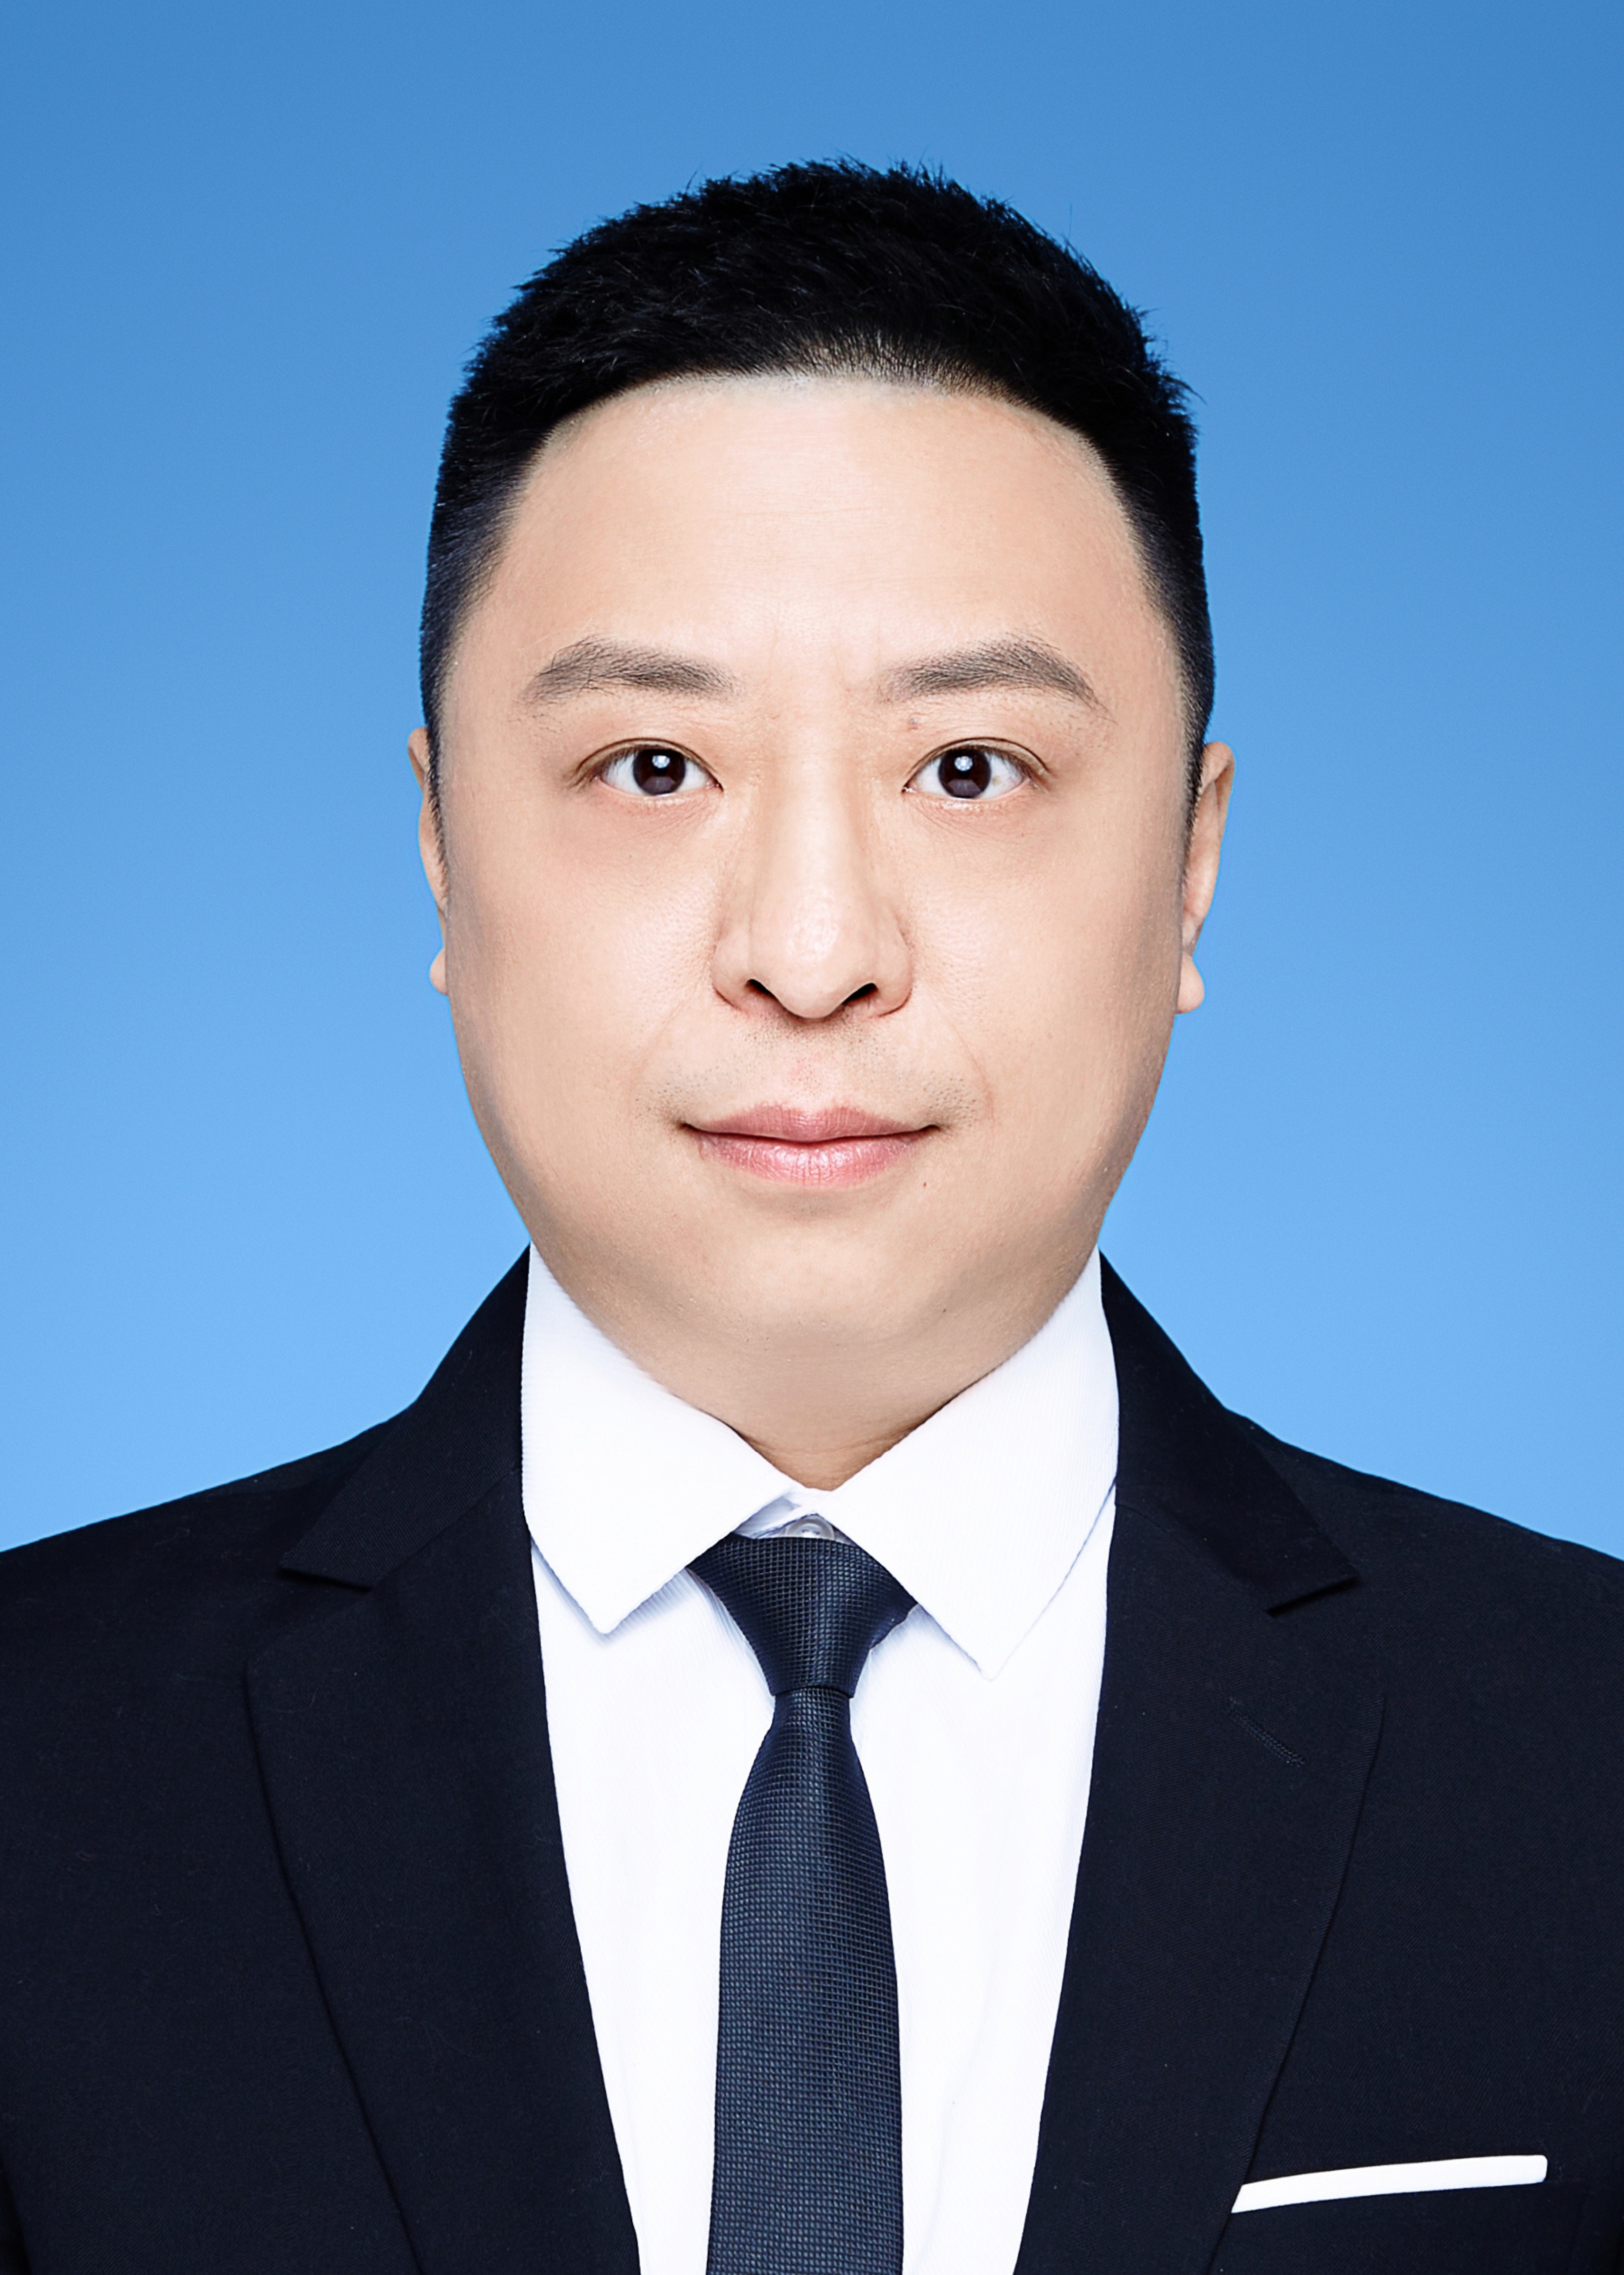
\includegraphics[width=1in,height=1.25in,clip,keepaspectratio]{bio_yehong_dong.pdf}}]{Yehong Dong}
is a professor with the School of New Energy, North China Electric Power University. He received the Ph.D. degree from Tsinghua University, Beijing, China, in 2011. His current research interests include wind turbine design and maintenance, machine learning, and AI-enhanced methods for failure diagnosis of wind power devices.
\end{IEEEbiography}

\begin{IEEEbiography}[{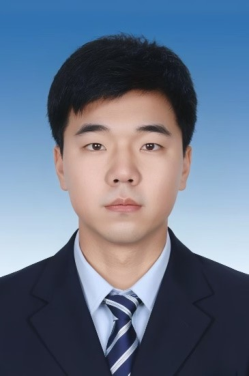
\includegraphics[width=1in,height=1.25in,clip,keepaspectratio]{bio_shuai_hao.pdf}}]{Shuai Hao}
received the B.S. degree from Beijing Institute of Technology, Beijing, China, in 2018, and the M.S. degree from Beihang University, Beijing, China, in 2022. He is currently pursuing the Ph.D. degree with the School of Automation Science and Electrical Engineering, Beihang University. His current research interests include knowledge graphs, retrieval-augmented generation, and large language models for industrial fault diagnosis.
\end{IEEEbiography}

\end{document}
